\documentclass{beamer}

\definecolor{myteal}{cmyk}{0.5,0,0.15,0}
\usecolortheme[named=myteal]{structure}

\usetheme{Madrid}
\usepackage{graphicx}
\usepackage{amsmath}
\usepackage{booktabs}
\usepackage{hyperref}
\usepackage{ctex}

\logo{\includegraphics[width=3cm]{LOGO.png}}


\title[BLIP-2 Presentation]{BLIP-2: Bootstrapping Language-Image Pre-training\\with Frozen Image Encoders and Large Language Models}
\author{王子恒 \newline SID:12310401}
\institute{SUSTech \newline CS308 Computer Vision \newline 期中论文汇报}
\date{2025年4月}

\begin{document}

\begin{frame}
  \titlepage
\end{frame}

\begin{frame}{目录}
  \tableofcontents
\end{frame}

\section{背景与动机}
\begin{frame}{背景与动机}
  \begin{itemize}
    \item 视觉-语言预训练(VLP)近年来迅速发展,在图像字幕生成、VQA等任务中表现突出
    \item 当前主流方法多采用端到端训练大型模型,资源消耗极高(如Flamingo80B参数达80B)
    \item 难以复用已有单模态模型(如CLIP, LLaMA, T5)
    \item \textbf{核心问题:如何高效桥接视觉和语言模态,降低训练开销?}
    \item BLIP-2 提出两阶段预训练框架,有效利用冻结的图像编码器和大语言模型(LLM)
  \end{itemize}
\end{frame}

\section{相关工作}
\begin{frame}{相关工作 I: 先行模型对比}
  \begin{itemize}
    \item \textbf{CLIP (Radford et al., 2021)}: 双塔结构,通过图文对比学习获取语义对齐特征
    \item \textbf{BLIP (Li et al., 2022)}: 引入多种预训练任务(ITC, ITM, ITG),强化图文建模
    \item \textbf{Frozen, Flamingo (2021-2022)}: 尝试将视觉特征注入冻结的LLM,实现图文生成
    \item 存在问题:模态对齐弱、训练成本高、参数量庞大
    \item BLIP-2 对比:\textbf{轻量Q-Former + 两阶段训练},兼顾效果与效率
  \end{itemize}
\end{frame}

\begin{frame}{相关工作 II: 基于BLIP-2的扩展研究}
  \textbf{InstructBLIP}\footnote{\href{https://arxiv.org/abs/2305.06500}{Dai et al., 2023}}:
  \begin{itemize}
    \item 将任务转换为指令格式训练
    \item 指令感知Q-Former增强泛化性
  \end{itemize}
  \includegraphics[width=0.85\linewidth]{instructblip.png}
  \vspace{1mm}
  
\end{frame}

\begin{frame}{相关工作 II: 基于BLIP-2的扩展研究}
    
\textbf{RegionBLIP}\footnote{\href{https://arxiv.org/abs/2308.02299}{Zhou et al., 2023}}:
  \begin{itemize}
    \item 面向区域目标的多模态扩展框架
  \end{itemize}
  \includegraphics[width=0.85\linewidth]{regionblip.pdf}
\end{frame}

\begin{frame}{相关工作 III: ChatCaptioner 图示}
  \textbf{ChatCaptioner}\footnote{\href{https://arxiv.org/abs/2303.06594}{Zhou et al., 2023}}:
  \begin{itemize}
    \item 通过ChatGPT提问循环,引导BLIP-2生成信息丰富的图像描述
    \item 自动多轮问答提升生成质量
  \end{itemize}
  \includegraphics[width=0.85\linewidth]{chatcaptioneroverview.png}
\end{frame}

\section{方法与创新}
\begin{frame}{BLIP-2整体架构}
  \centering
  \includegraphics[width=0.9\textwidth]{image/fig1-example.pdf}
  \vspace{0.3cm}
  \\
  \small{BLIP-2通过Q-Former连接冻结的视觉编码器和语言模型}
\end{frame}

\begin{frame}{Q-Former: 核心创新}
  \begin{itemize}
    \item \textbf{功能}:作为视觉编码器和语言模型之间的桥梁
    \item \textbf{结构}:
      \begin{itemize}
        \item 包含两组输入:图像特征和查询嵌入(query embeddings)
        \item 基于Transformer架构,采用交叉注意力机制
        \item 查询嵌入可学习,通过注意力从图像特征中提取关键信息
      \end{itemize}
    \item \textbf{优势}:
      \begin{itemize}
        \item 减少参数数量,降低计算成本
        \item 实现高效信息提取和模态对齐
        \item 可灵活连接不同规模的语言模型
      \end{itemize}
  \end{itemize}
\end{frame}

\begin{frame}{Q-Former详细结构}
    \centering
    \includegraphics[width=0.8\textwidth]{image/fig2-v2.pdf}
    \vspace{0.2cm}
    \\
    \caption{Q-Former的内部结构与注意力机制}
  \end{frame}

\begin{frame}{两阶段预训练策略}
    \centering
    \textbf{第一阶段:表征学习}
    \begin{itemize}
        \item 冻结ViT图像编码器
        \item 训练Q-Former理解视觉信息
        \item 使用三个目标函数:
            \begin{itemize}
                \item 图像-文本对比学习
                \item 图像-文本匹配
                \item 图像条件文本生成
            \end{itemize}
    \end{itemize}
    \vspace{0.5cm}
    \includegraphics[width=0.8\textwidth]{image/fig2-v5.pdf}
    \\
    \caption*{第一阶段的预训练任务}
\end{frame}

\begin{frame}{两阶段预训练策略}
    \centering
    \textbf{第二阶段:指令调优}
    \begin{itemize}
        \item 冻结第一阶段训练的Q-Former
        \item 冻结预训练LLM
        \item 只训练一个线性投影层
        \item 将视觉特征转换为LLM可理解的表示
        \item 使用指令数据集微调
    \end{itemize}
    \vspace{0.5cm}
    \includegraphics[width=0.8\textwidth]{image/fig3-v3.pdf}
    \\
    \caption*{第二阶段的预训练任务}
\end{frame}



\section{实验结果与分析}

  \begin{frame}{实验设置概述}
    \begin{itemize}
      \item \textbf{预训练数据}:1.4亿图像-文本对
      \item \textbf{视觉编码器}:ViT-L/14和ViT-G (从CLIP预训练)
      \item \textbf{语言模型}:
        \begin{itemize}
          \item 指令调优型: Flan-T5 (XL和XXL)
          \item 无监督型: OPT (2.7B和6.7B)
        \end{itemize}
      \item \textbf{评估任务}:视觉问答、图像字幕生成、图像-文本检索、零样本生成能力
    \end{itemize}
  \end{frame}
  
  \begin{frame}{零样本视觉语言任务性能}
    \centering
    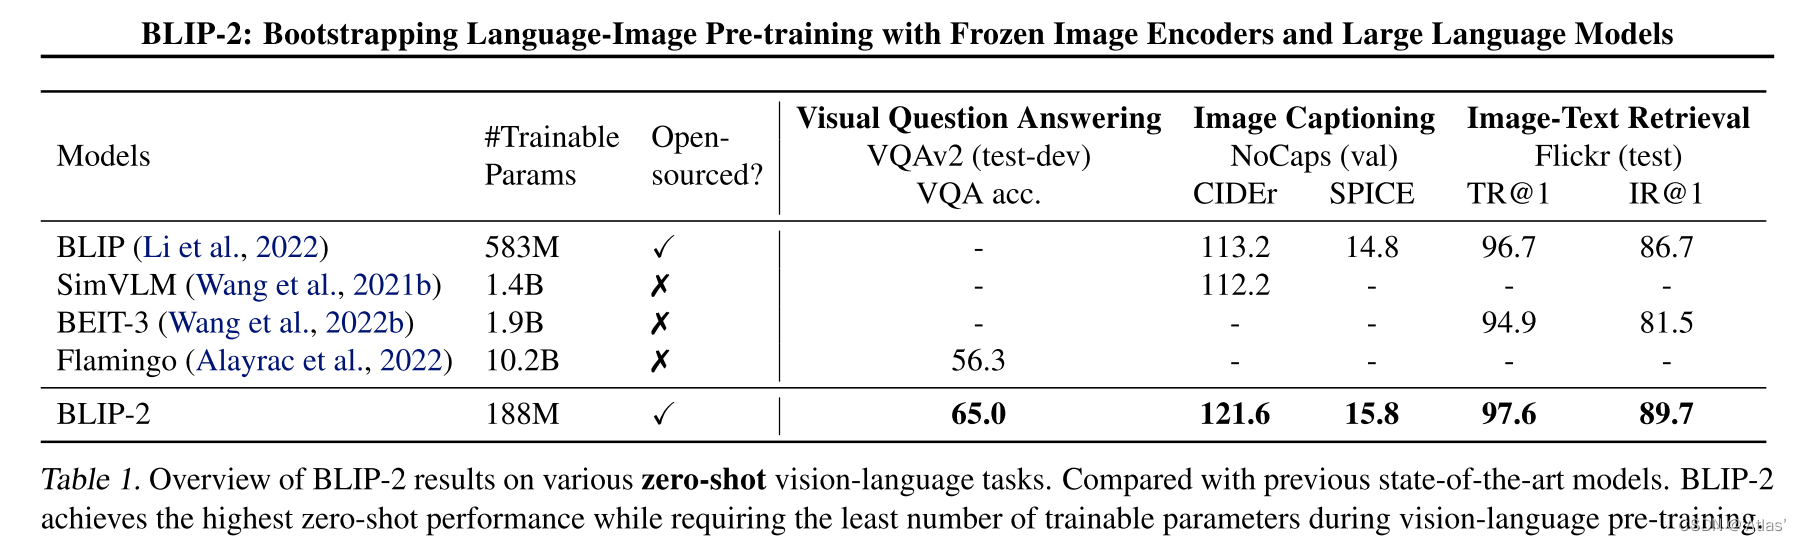
\includegraphics[width=0.85\textwidth]{table1.png}
    \vspace{0.2cm}
    
    \begin{itemize}
      \item BLIP-2达到或超越SOTA性能,同时训练参数量显著减少
      \item Flamingo训练80B参数,而BLIP-2只需训练188M参数
      \item 通过复用预训练模型能力,大幅提高参数效率
    \end{itemize}
  \end{frame}
  
  \begin{frame}{零样本图像到文本生成能力}
    \centering
    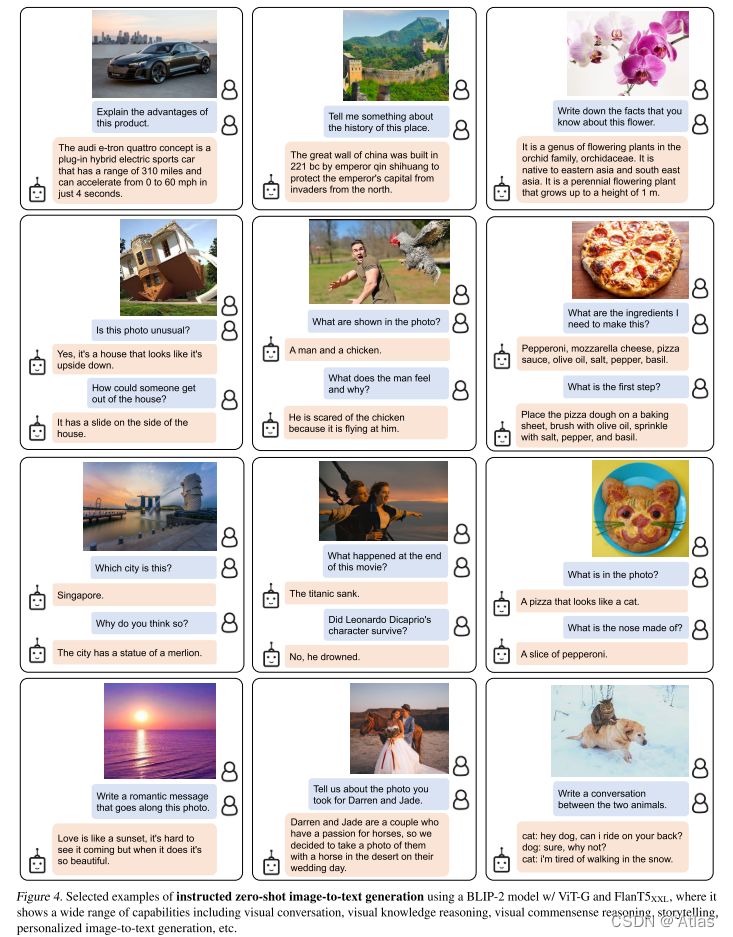
\includegraphics[width=0.9\textwidth]{table2.png}
    \vspace{0.2cm}
    
    \begin{itemize}
      \item BLIP-2展示了多种零样本生成能力:
        \begin{itemize}
          \item 视觉知识推理:理解图像中的物体、场景和关系
          \item 视觉共鸣推理:推断图像中隐含的信息和背景
          \item 视觉对话:基于图像进行多轮对话交流
          \item 个性化图像描述:根据提示风格生成描述
        \end{itemize}
      \item 结合了LLM的文本指令遵循能力与图像理解能力
    \end{itemize}
  \end{frame}
  
  \begin{frame}{零样本VQA性能分析}
    \centering
    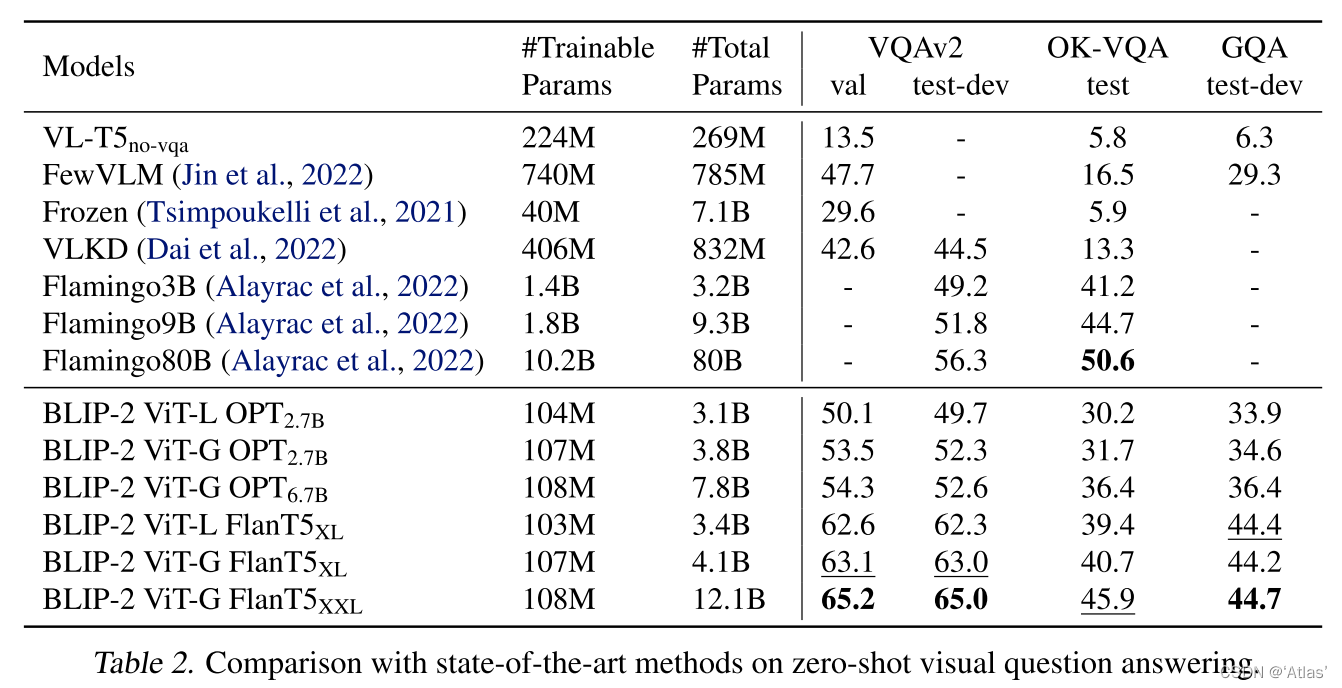
\includegraphics[width=0.85\textwidth]{table3.png}
    \vspace{0.2cm}
    
    \begin{itemize}
      \item 关键发现:
        \begin{itemize}
          \item 更强的图像编码器或更大的LLM都能提升BLIP-2性能
          \item 指令调优的FlanT5显著优于无监督的OPT
          \item ViT-G + FlanT5-XXL组合取得最佳性能:VQAv2达65.0\%,GQA达44.7\%
        \end{itemize}
      \item 证明了BLIP-2架构的灵活性和可扩展性
    \end{itemize}
  \end{frame}
  
  \begin{frame}{表征学习的重要性}
    \centering
    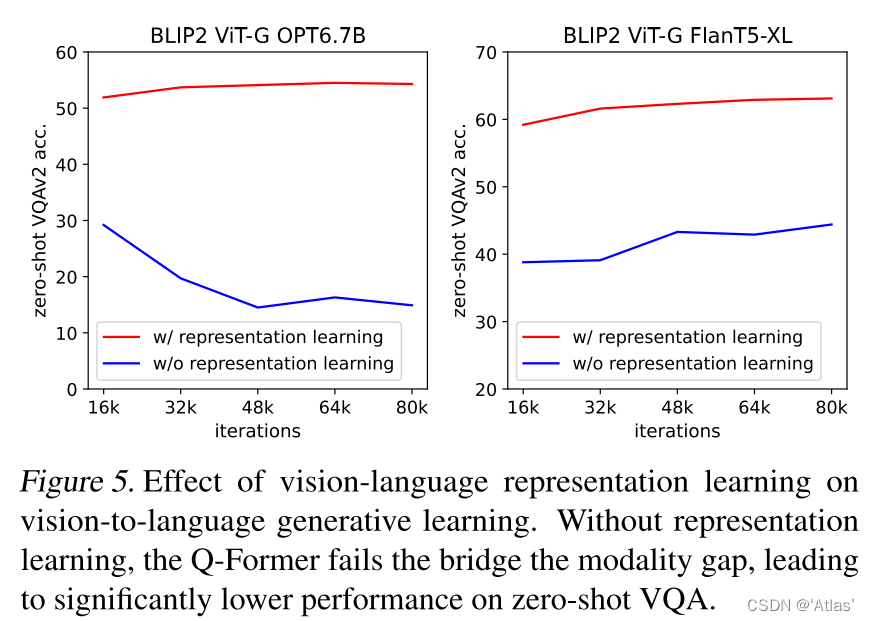
\includegraphics[width=0.6\textwidth]{table4.png}
    \vspace{0.2cm}
    
    \begin{itemize}
      \item 第一阶段预训练使Q-Former学习提取与文本相关的视觉表征
      \item 消融实验结果:
        \begin{itemize}
          \item 没有表征学习阶段,两种LLM在零样本VQA任务性能大幅下降
          \item OPT模型性能从50\%降至30\%甚至10\%,下降20个百分点以上
          \item FlanT5模型性能从60\%降至40\%,下降约20个百分点
        \end{itemize}
      \item 证明两阶段训练策略的有效性和必要性
    \end{itemize}
  \end{frame}
  
  \begin{frame}{图像描述生成结果}
    \centering
    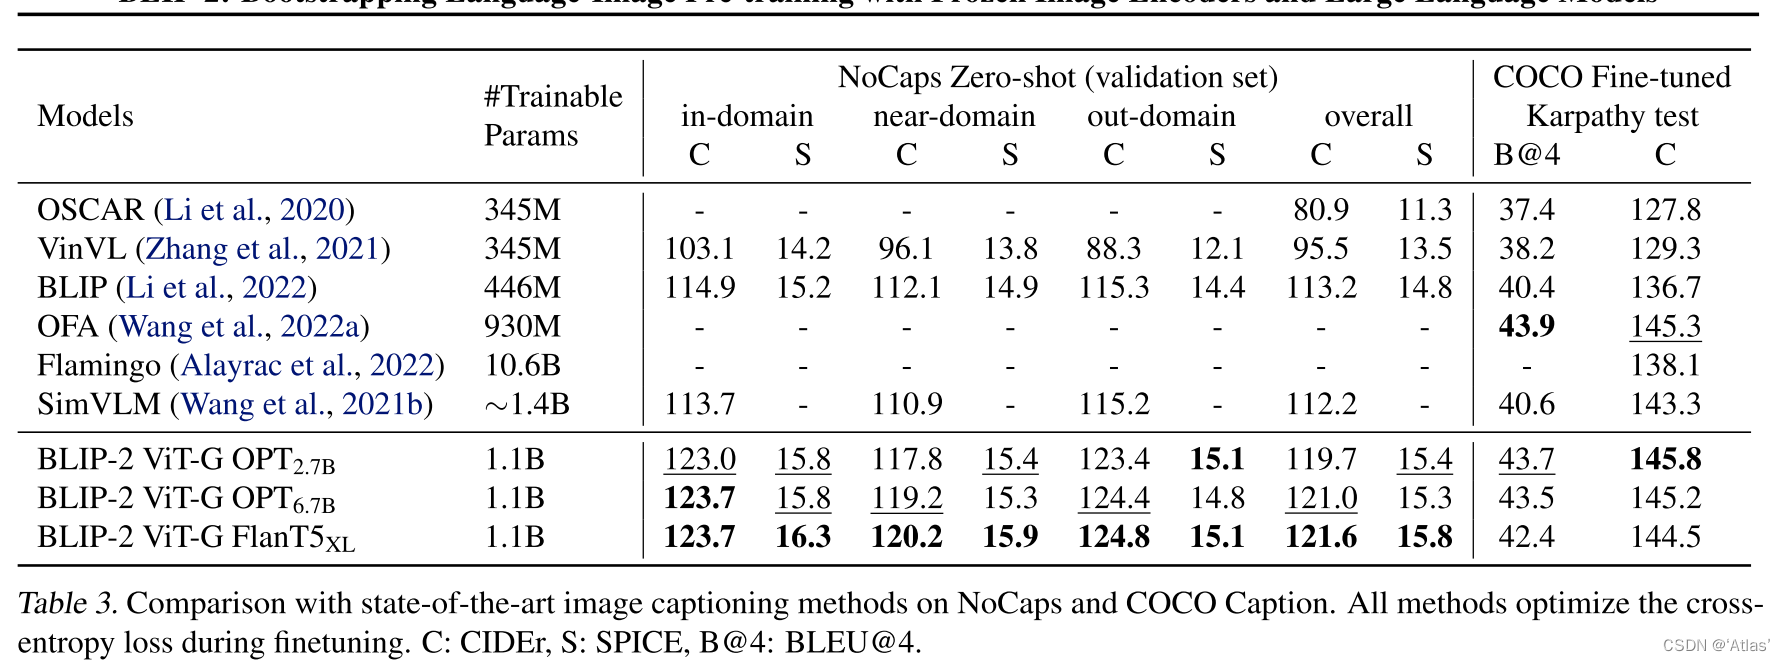
\includegraphics[width=0.85\textwidth]{table5.png}
    \vspace{0.2cm}
    
    \begin{itemize}
      \item BLIP-2在COCO和NoCaps数据集上均达到SOTA性能:
        \begin{itemize}
          \item COCO: 145.8 CIDEr分数
          \item NoCaps: 15.8 CIDEr分数
        \end{itemize}
      \item 在NoCaps上的优异表现展示了强大的跨域生成能力
      \item 能够准确描述训练中未见过的对象和场景
    \end{itemize}
  \end{frame}
  
  \begin{frame}{视觉问答任务分析}
    \centering
    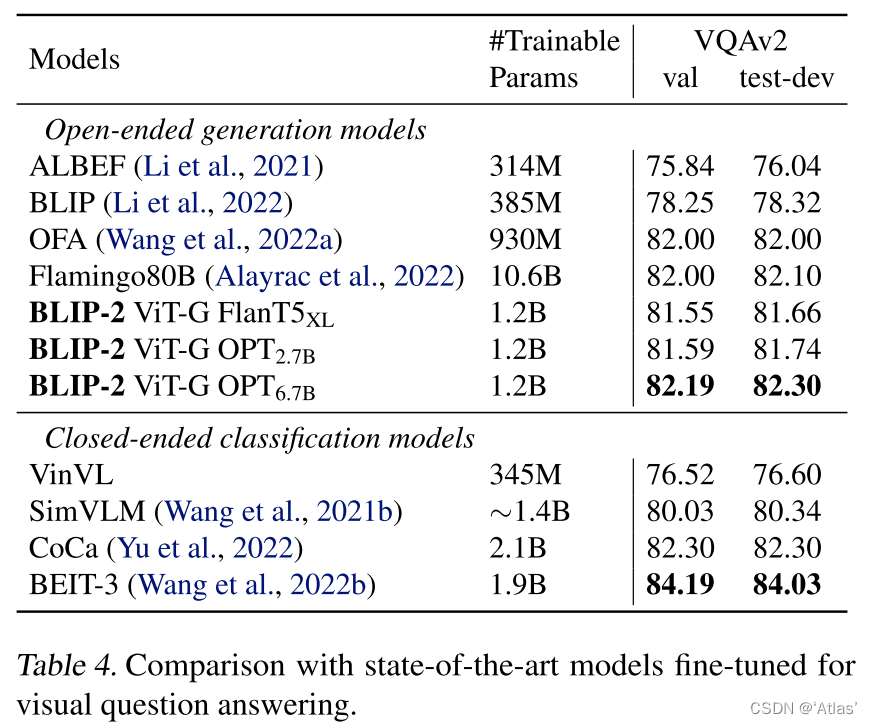
\includegraphics[width=0.5\textwidth]{table6.png}
    \vspace{0.2cm}
    
    \begin{itemize}
      \item \textbf{创新输入处理方式}:
        \begin{itemize}
          \item 问题文本输入到Q-Former,引导关注图像相关区域
          \item 通过self-attention机制,query与问题交互
          \item cross-attention关注图像中与问题相关的区域
        \end{itemize}
      \item \textbf{结果}:在开放式生成模型中达到SOTA表现
    \end{itemize}
  \end{frame}
  
  \begin{frame}{图像文本检索性能}
    \centering
    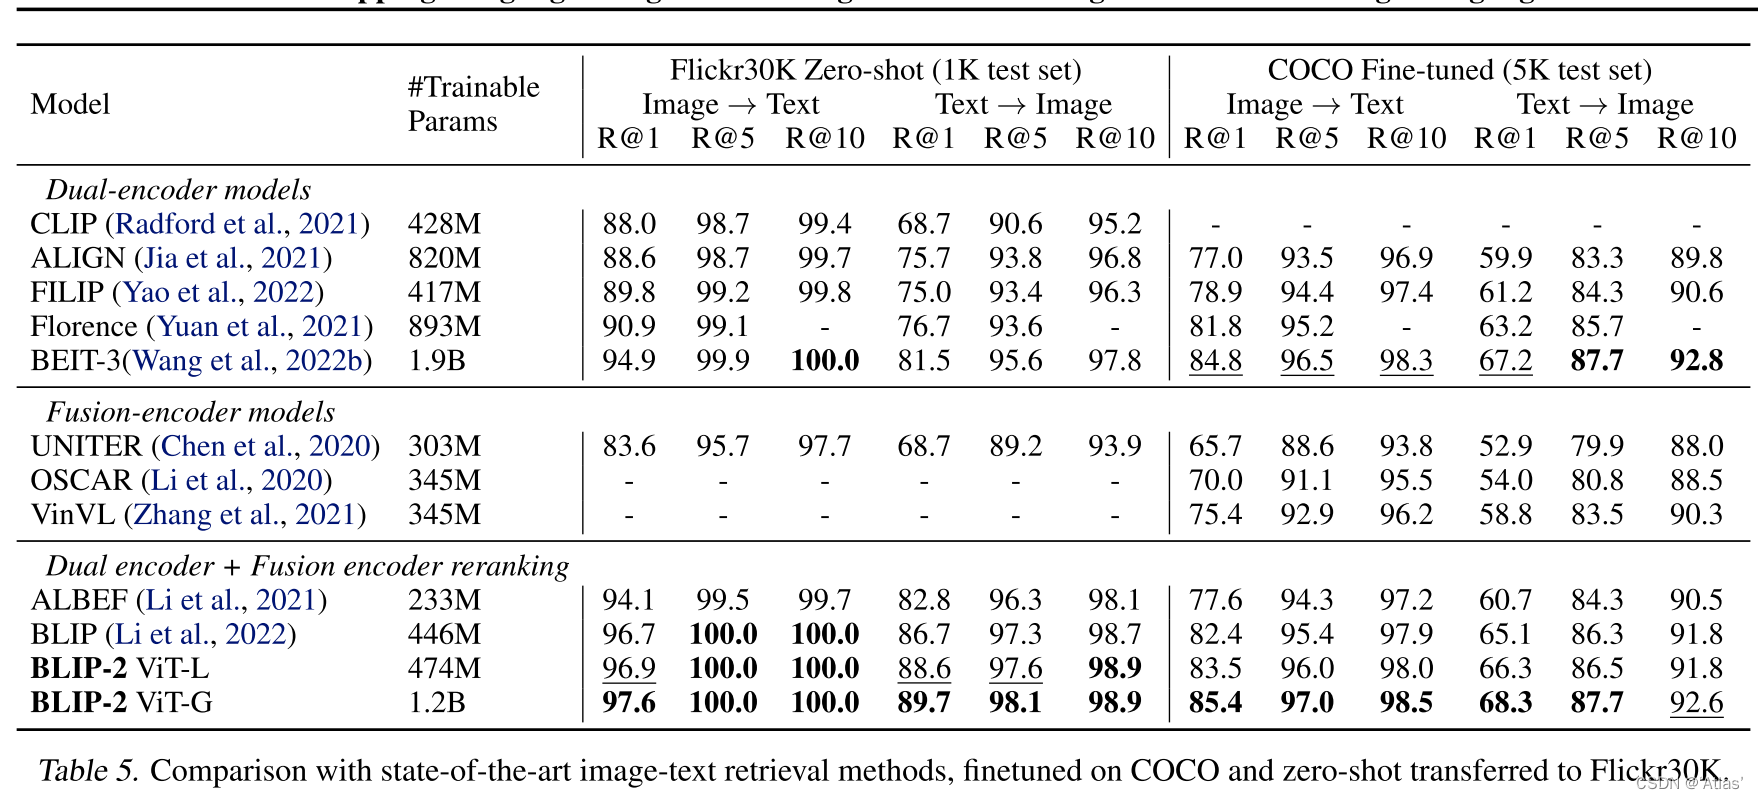
\includegraphics[width=0.85\textwidth]{table7.png}
    \vspace{0.2cm}
    
    \begin{itemize}
      \item 检索过程:先根据相似度选128个候选,再根据ITM分数排序
      \item BLIP-2在COCO和Flickr30K上均显著超越之前方法:
        \begin{itemize}
          \item COCO图像→文本检索:85.4\% (vs. BLIP的82.4\%)
          \item Flickr30K文本→图像检索:89.7\% (vs. BLIP的86.7\%)
        \end{itemize}
    \end{itemize}
  \end{frame}
  
  \begin{frame}{实验结果总结}
    \begin{itemize}
      \item \textbf{关键发现}:
        \begin{itemize}
          \item BLIP-2在各类视觉-语言任务上都取得SOTA或接近SOTA性能
          \item 通过冻结预训练模型,极大降低训练参数量和计算成本
          \item 视觉编码器和语言模型质量对BLIP-2性能有直接影响
          \item 两阶段预训练策略对模型性能至关重要
        \end{itemize}
      \item \textbf{优势}:
        \begin{itemize}
          \item 参数效率高:仅训练188M参数即可达到优异性能
          \item 灵活性:可与不同规模视觉和语言模型结合
          \item 泛化能力强:在跨域和零样本任务中表现突出
        \end{itemize}
    \end{itemize}
  \end{frame}

  \section{个人见解与延伸思考}

 \begin{frame}{局限性分析}
  \begin{itemize}
    \item \textbf{技术层面局限}:
      \begin{itemize}
        \item 对视觉编码器质量的强依赖性
        \item Q-Former可能成为信息瓶颈
        \item 难以处理超出ViT预训练范围的视觉场景
        \item 对时序信息和空间关系建模不足
      \end{itemize}
    \item \textbf{应用层面挑战}:
      \begin{itemize}
        \item 上下文理解有限,难以把握复杂场景
        \item 在专业领域(如医学、科学图像)表现不佳
        \item 与人类偏好的对齐问题
        \item 缺乏多模态的知识推理能力
      \end{itemize}
    \item \textbf{潜在的社会影响}:
      \begin{itemize}
        \item 可能继承预训练模型中的偏见和刻板印象
        \item 对隐私和版权内容的识别与生成问题
      \end{itemize}
  \end{itemize}
\end{frame}

\begin{frame}{后续研究方向与可能的突破点}
    \begin{columns}
      \column{0.5\textwidth}
      \textbf{架构改进}
      \begin{itemize}
        \item 动态适应的Q-Former,根据任务调整查询数
        \item 多级别视觉特征融合(局部+全局)
        \item 探索Perceiver-IO等替代架构
        \item 将Transformer替换为更高效结构
      \end{itemize}
      
      \column{0.5\textwidth}
      \textbf{训练与应用}
      \begin{itemize}
        \item 整合多源知识(如常识、关系等)
        \item 强化学习用于优化视觉特征选择
        \item 探索连续学习方法适应新模态
        \item 用于生成具身AI的视觉基础
      \end{itemize}
    \end{columns}
    
    \vspace{0.3cm}
    \textbf{个人观点}:未来视觉-语言模型的关键在于\textbf{高效适应性连接}而非模型规模。BLIP-2的思路比纯粹扩大模型更有前途。
  \end{frame}

\section{结论与未来工作}
\begin{frame}{结论与未来工作}
  \begin{itemize}
    \item \textbf{主要贡献}:
      \begin{itemize}
        \item 提出Q-Former架构,高效连接视觉和语言模型
        \item 实现参数高效的预训练策略,显著降低计算成本
        \item 在多项视觉-语言任务上取得SOTA结果
      \end{itemize}
    \item \textbf{局限性}:
      \begin{itemize}
        \item 对特定领域知识的理解仍有不足
        \item 在某些复杂推理任务上表现不稳定
      \end{itemize}
    \item \textbf{未来工作}:
      \begin{itemize}
        \item 扩展到视频、3D等多模态数据
        \item 增强模型的推理和知识整合能力
        \item 研究更高效的模态对齐和融合方法
      \end{itemize}
  \end{itemize}
\end{frame}

\begin{frame}{参考文献}
  \begin{thebibliography}{9}
    \bibitem{blip2} Li, J. et al. (2023). BLIP-2: Bootstrapping Language-Image Pre-training with Frozen Image Encoders and Large Language Models. arXiv preprint arXiv:2301.12597.
    \bibitem{clip} Radford, A. et al. (2021). Learning Transferable Visual Models From Natural Language Supervision. ICML 2021.
    \bibitem{flamingo} Alayrac, J. et al. (2022). Flamingo: a Visual Language Model for Few-Shot Learning. NeurIPS 2022.
  \end{thebibliography}
\end{frame}

\begin{frame}
  \centering
  \LARGE{谢谢观看!}
  \vspace{1cm}
\end{frame}


\end{document}
